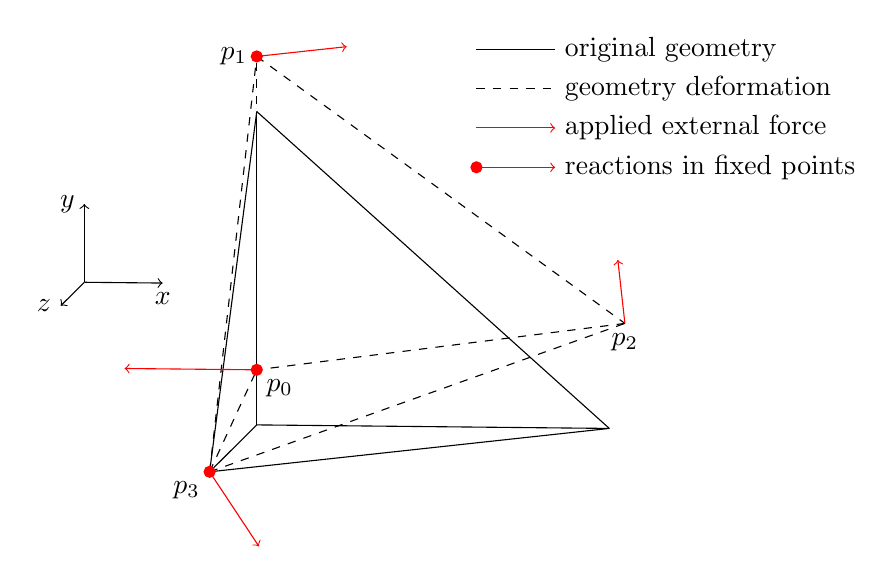
\begin{tikzpicture}
\draw[->] (-0.980017,2.03987) -- (0.0149875,2.0299);
\node[below] at (0.0149875,2.0299) {$x$};
\draw[->] (-0.980017,2.03987) -- (-0.980017,3.03487);
\node[left] at (-0.980017,3.03487) {$y$};
\draw[->] (-0.980017,2.03987) -- (-1.27952,1.74186);
\node[left] at (-1.27952,1.74186) {$z$};
\draw (1.20966,0.228594) -- (1.20966,4.20861);
\draw (1.20966,4.20861) -- (5.68718,0.183744);
\draw (5.68718,0.183744) -- (1.20966,0.228594);
\draw (0.610658,-0.367414) -- (1.20966,0.228594);
\draw (0.610658,-0.367414) -- (1.20966,4.20861);
\draw (0.610658,-0.367414) -- (5.68718,0.183744);
\draw[dashed] (1.20966,0.928164) -- (1.20966,4.90818);
\draw[dashed] (1.20966,4.90818) -- (5.88499,1.51754);
\draw[dashed] (5.88499,1.51754) -- (1.20966,0.928164);
\draw[dashed] (0.610658,-0.367414) -- (1.20966,0.928164);
\draw[dashed] (0.610658,-0.367414) -- (1.20966,4.90818);
\draw[dashed] (0.610658,-0.367414) -- (5.88499,1.51754);
\draw[fill,red] (1.20966,0.928164) circle(0.07);
\draw[->,red] (1.20966,0.928164) -- (-0.469411,0.944983);
\node[below right] at (1.20966,0.928164) {$p_0$};
\draw[fill,red] (1.20966,4.90818) circle(0.07);
\draw[->,red] (1.20966,4.90818) -- (2.35188,5.03219);
\node[left] at (1.20966,4.90818) {$p_1$};
\draw[->,red] (5.88499,1.51754) -- (5.79514,2.32364);
\node[below] at (5.88499,1.51754) {$p_2$};
\draw[fill,red] (0.610658,-0.367414) circle(0.07);
\draw[->,red] (0.610658,-0.367414) -- (1.23736,-1.31435);
\node[below left] at (0.610658,-0.367414) {$p_3$};
\draw (4,5) -- (5,5);
\node[right] at (5,5) {original geometry};
\draw[dashed] (4,4.5) -- (5,4.5);
\node[right] at (5,4.5) {geometry deformation};
\draw[->,red] (4,4) -- (5,4);
\node[right] at (5,4) {applied external force};
\draw[->,red] (4,3.5) -- (5,3.5);
\node[right] at (5,3.5) {reactions in fixed points};
\draw[fill,red] (4,3.5) circle(0.07);
\end{tikzpicture}